\subsection{User Study}~\label{exp:user_study}
We conducted a Wizard-of-Oz (WoZ) user study to evaluate how different query policies affect user responses, interaction time, subjective workload, and situation awareness during human--robot collaboration. Unlike the system evaluation in Section~\ref{exp:sys_eval}, which focused on autonomous task performance, this study focused on the user-side effect of different interaction strategies. Robot behavior was controlled using predefined scenario scripts, while participants interacted with the system through the same tablet-based interface used by the feedback manager.

\subsubsection{Participants}~\label{user:participants}

Twelve participants (7 female and 5 male) took part in the study. Participants ranged in age from 21 to 26 years ($M=23.0$, $SD=1.48$). Each participant received \$20 upon completion of the study.

\subsubsection{Study Design and Conditions}~\label{user:design}

The study employed a within-subject design. Each participant completed ten trials in total, consisting of five waste sorting scenarios and five tomato harvesting scenarios. In each domain, participants experienced five interaction conditions: \textbf{All}, \textbf{No}, \textbf{Ours1}, \textbf{Ours2}, and \textbf{KnowNo}. \textbf{All} requested feedback whenever a query was available, representing continuous human supervision. \textbf{No} performed the task without requesting user feedback. \textbf{Ours1} used the proposed uncertainty-based state query policy. \textbf{Ours2} used a variant of the proposed policy designed to expose participants to a broader range of query situations. \textbf{KnowNo} served as an action-level query baseline.

Each domain consisted of five scenarios and five interaction conditions. The assignment between scenarios and conditions was randomized for each participant such that every participant experienced all five conditions exactly once per domain. This design prevented a particular condition from being consistently associated with a specific scenario. Detailed scenario descriptions are provided in Appendix~\ref{appx:user}.

\subsubsection{Materials and Procedure}~\label{user:materials_procedure}

Participants interacted with the robot through a tablet-based interface. The interface displayed the current task state, highlighted task-relevant objects, and presented robot-generated questions together with selectable answer options. The waste sorting scenarios required participants to identify the category of waste objects, including general waste, paper, cans, and plastic. The tomato harvesting scenarios required participants to identify the state of tomatoes, such as whether a tomato was ripe, unripe, or rotten.

Before the experiment, participants received an explanation of the study objectives, the two task domains, and the robot interaction process. They were then introduced to the tablet interface and completed practice interactions to become familiar with the available information and response procedure. During the main session, participants completed ten trials without assistance. If a participant selected an incorrect answer, the response was recorded as incorrect for evaluation purposes, but the scenario continued using the intended task state so that subsequent interactions were not affected by earlier mistakes. After each scenario, participants completed a questionnaire regarding the interaction experience. After completing all ten trials, participants completed post-study questionnaires and provided qualitative feedback during a short debriefing session.

\subsubsection{Measures}~\label{user:measures}

We organized the user-study analysis along three axes. First, we evaluated response quality using scenario--condition answer accuracy and task success. Answer accuracy measures whether each user response matched the predefined answer key. Task success is stricter: a task is counted as successful only when all required answers in that task were correct. Because \textbf{No} does not request user answers, it is not scored in this response-quality analysis.

Second, we measured time cost. Operation time was computed from the recorded timeline after subtracting the scenario video duration, so that the value reflects pure user operation time rather than passive viewing time. Survey time was measured separately. Missing scenario--condition cells were retained as empty cells in the summary tables and excluded from mean calculations.

Third, we analyzed subjective and situation-awareness measures. Subjective workload was measured using NASA Raw-TLX. Situation awareness was evaluated using SAGAT-style questions and SART. Cognitive fatigue was measured using a self-reported fatigue item. Unless otherwise specified, questionnaire responses were recorded using a 5-point Likert scale. For the within-subject questionnaire analysis, we used Friedman tests across the five conditions and planned exact Wilcoxon signed-rank tests centered on \textbf{Ours1} and \textbf{Ours2}, with Holm correction within each measure and domain panel.

\subsubsection{Results: Response Accuracy and Task Success}~\label{user:results_op_sr}

Fig.~\ref{fig:user_response_quality} summarizes the response-quality results across both domains. In answer-level accuracy, \textbf{All}, \textbf{Ours1}, and \textbf{Ours2} generally remained high across scenarios, whereas \textbf{KnowNo} decreased in the later scenarios. For example, in Scenario~4, answer accuracy was $98.5\%$ for \textbf{All}, $89.7\%$ for \textbf{Ours1}, $97.5\%$ for \textbf{Ours2}, and $66.7\%$ for \textbf{KnowNo}. In Scenario~5, \textbf{Ours1} reached $100.0\%$, \textbf{Ours2} reached $93.3\%$, and \textbf{KnowNo} reached $73.3\%$.

\begin{figure*}[t]
    \centering
    \begin{subfigure}[t]{0.48\textwidth}
        \centering
        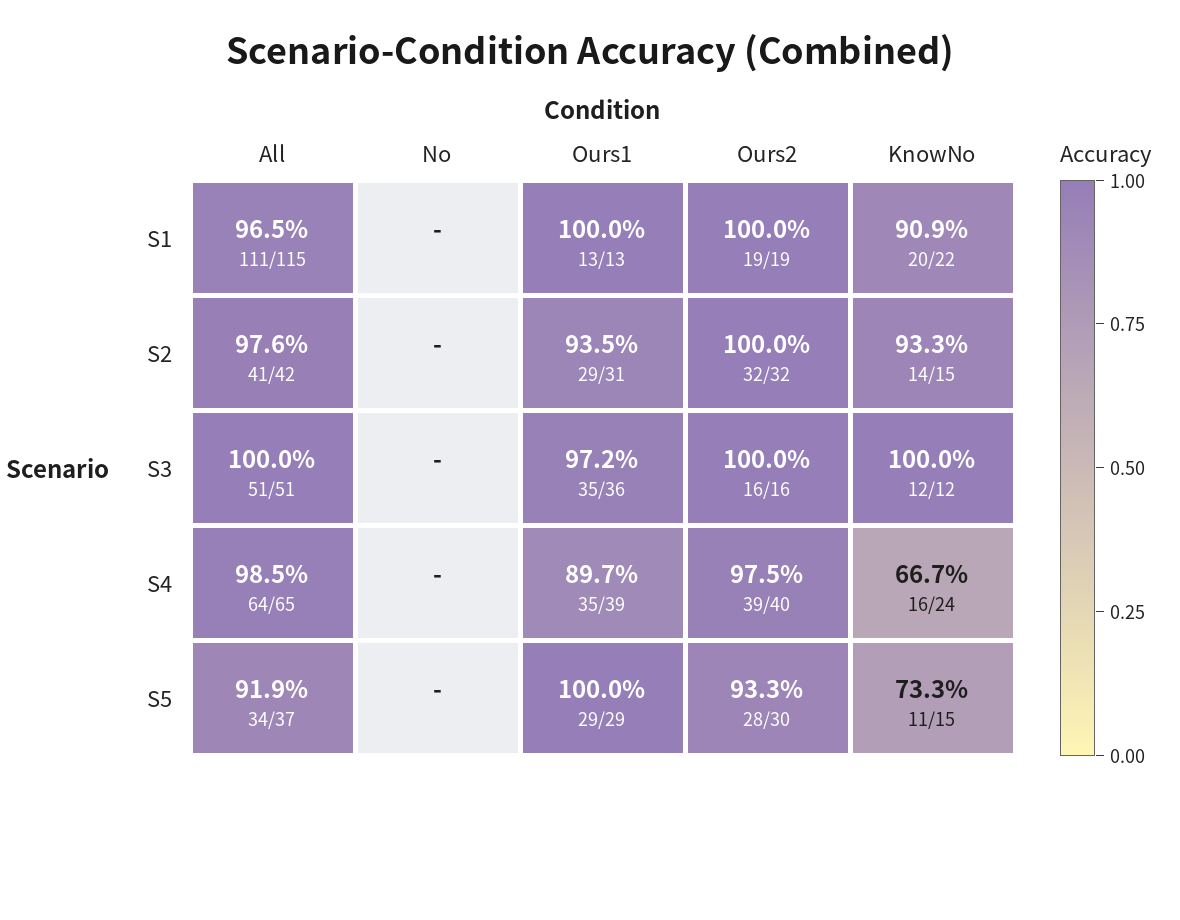
\includegraphics[width=\linewidth]{figures/fig_user_accuracy_combined.png}
        \caption{Answer-level accuracy.}
        \label{fig:user_answer_accuracy}
    \end{subfigure}
    \hfill
    \begin{subfigure}[t]{0.48\textwidth}
        \centering
        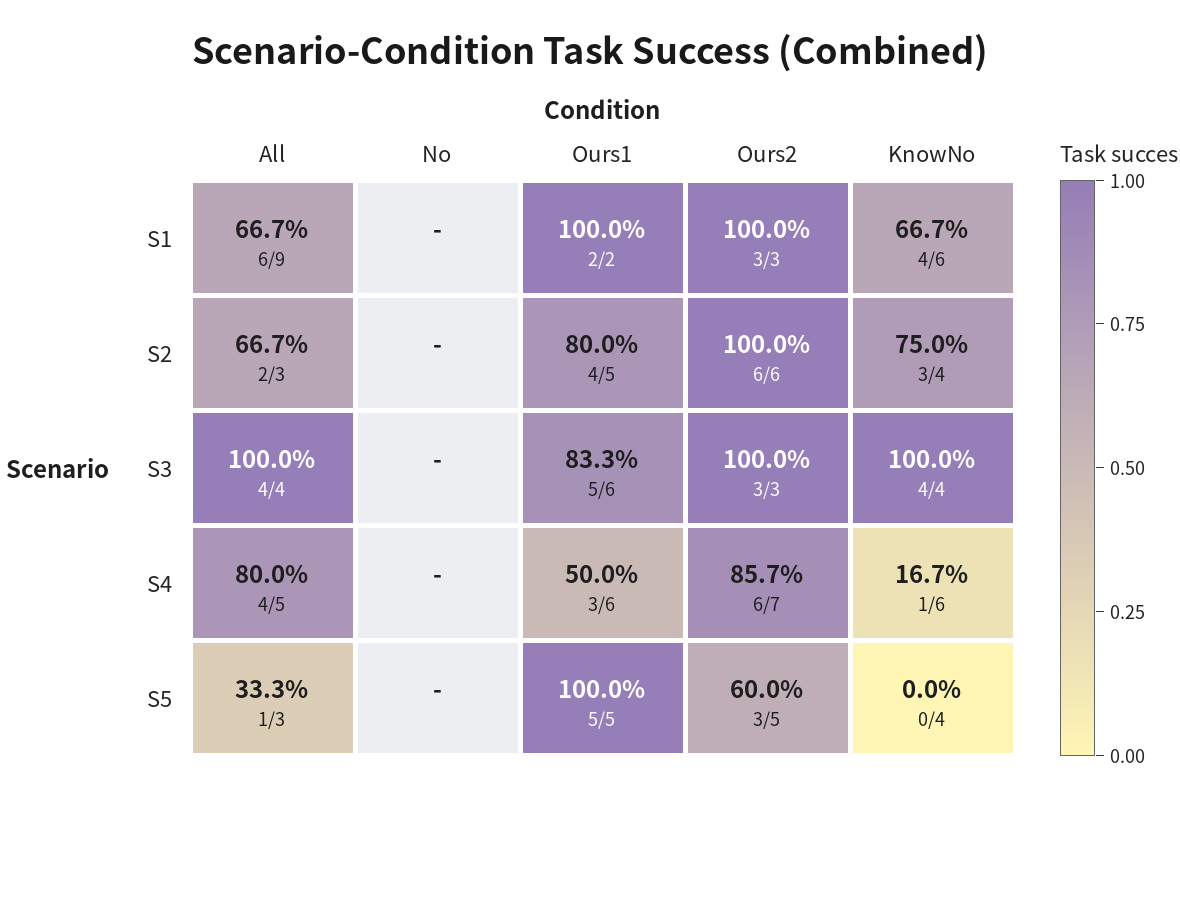
\includegraphics[width=\linewidth]{figures/fig_user_task_success_combined.png}
        \caption{Task-level success.}
        \label{fig:user_task_success}
    \end{subfigure}
    \caption{Response-quality results by scenario and condition. Answer accuracy scores individual responses, whereas task success counts a task as successful only if all required answers were correct. Blank cells indicate conditions that did not produce scorable user responses.}
    \label{fig:user_response_quality}
\end{figure*}

The stricter task-success metric shows the cost of individual mistakes more clearly. \textbf{Ours2} achieved perfect task success in Scenarios~1--3 and remained high in Scenario~4 ($85.7\%$), while \textbf{KnowNo} dropped to $16.7\%$ in Scenario~4 and $0.0\%$ in Scenario~5. \textbf{Ours1} showed perfect task success in Scenarios~1 and~5, but decreased in Scenario~4 ($50.0\%$). These results suggest that state-level queries can support accurate user responses, but the benefit depends on the scenario and on how the query distribution interacts with task difficulty.

\subsubsection{Results: Operation and Survey Time}~\label{user:results_time}

Fig.~\ref{fig:user_time_results} summarizes pure operation time and survey time for the two domains. After subtracting scenario video duration, \textbf{No} had the shortest pure operation time, as expected, because it did not require user responses. In waste sorting, the mean pure operation time across available scenarios was $0.44$~s for \textbf{No}, $6.90$~s for \textbf{Ours1}, $7.87$~s for \textbf{Ours2}, $20.31$~s for \textbf{KnowNo}, and $22.19$~s for \textbf{All}. In tomato harvesting, the corresponding values were $1.78$~s for \textbf{No}, $14.27$~s for \textbf{Ours1}, $13.98$~s for \textbf{Ours2}, $25.33$~s for \textbf{KnowNo}, and $23.60$~s for \textbf{All}.

\begin{figure*}[t]
    \centering
    \begin{subfigure}[t]{0.49\textwidth}
        \centering
        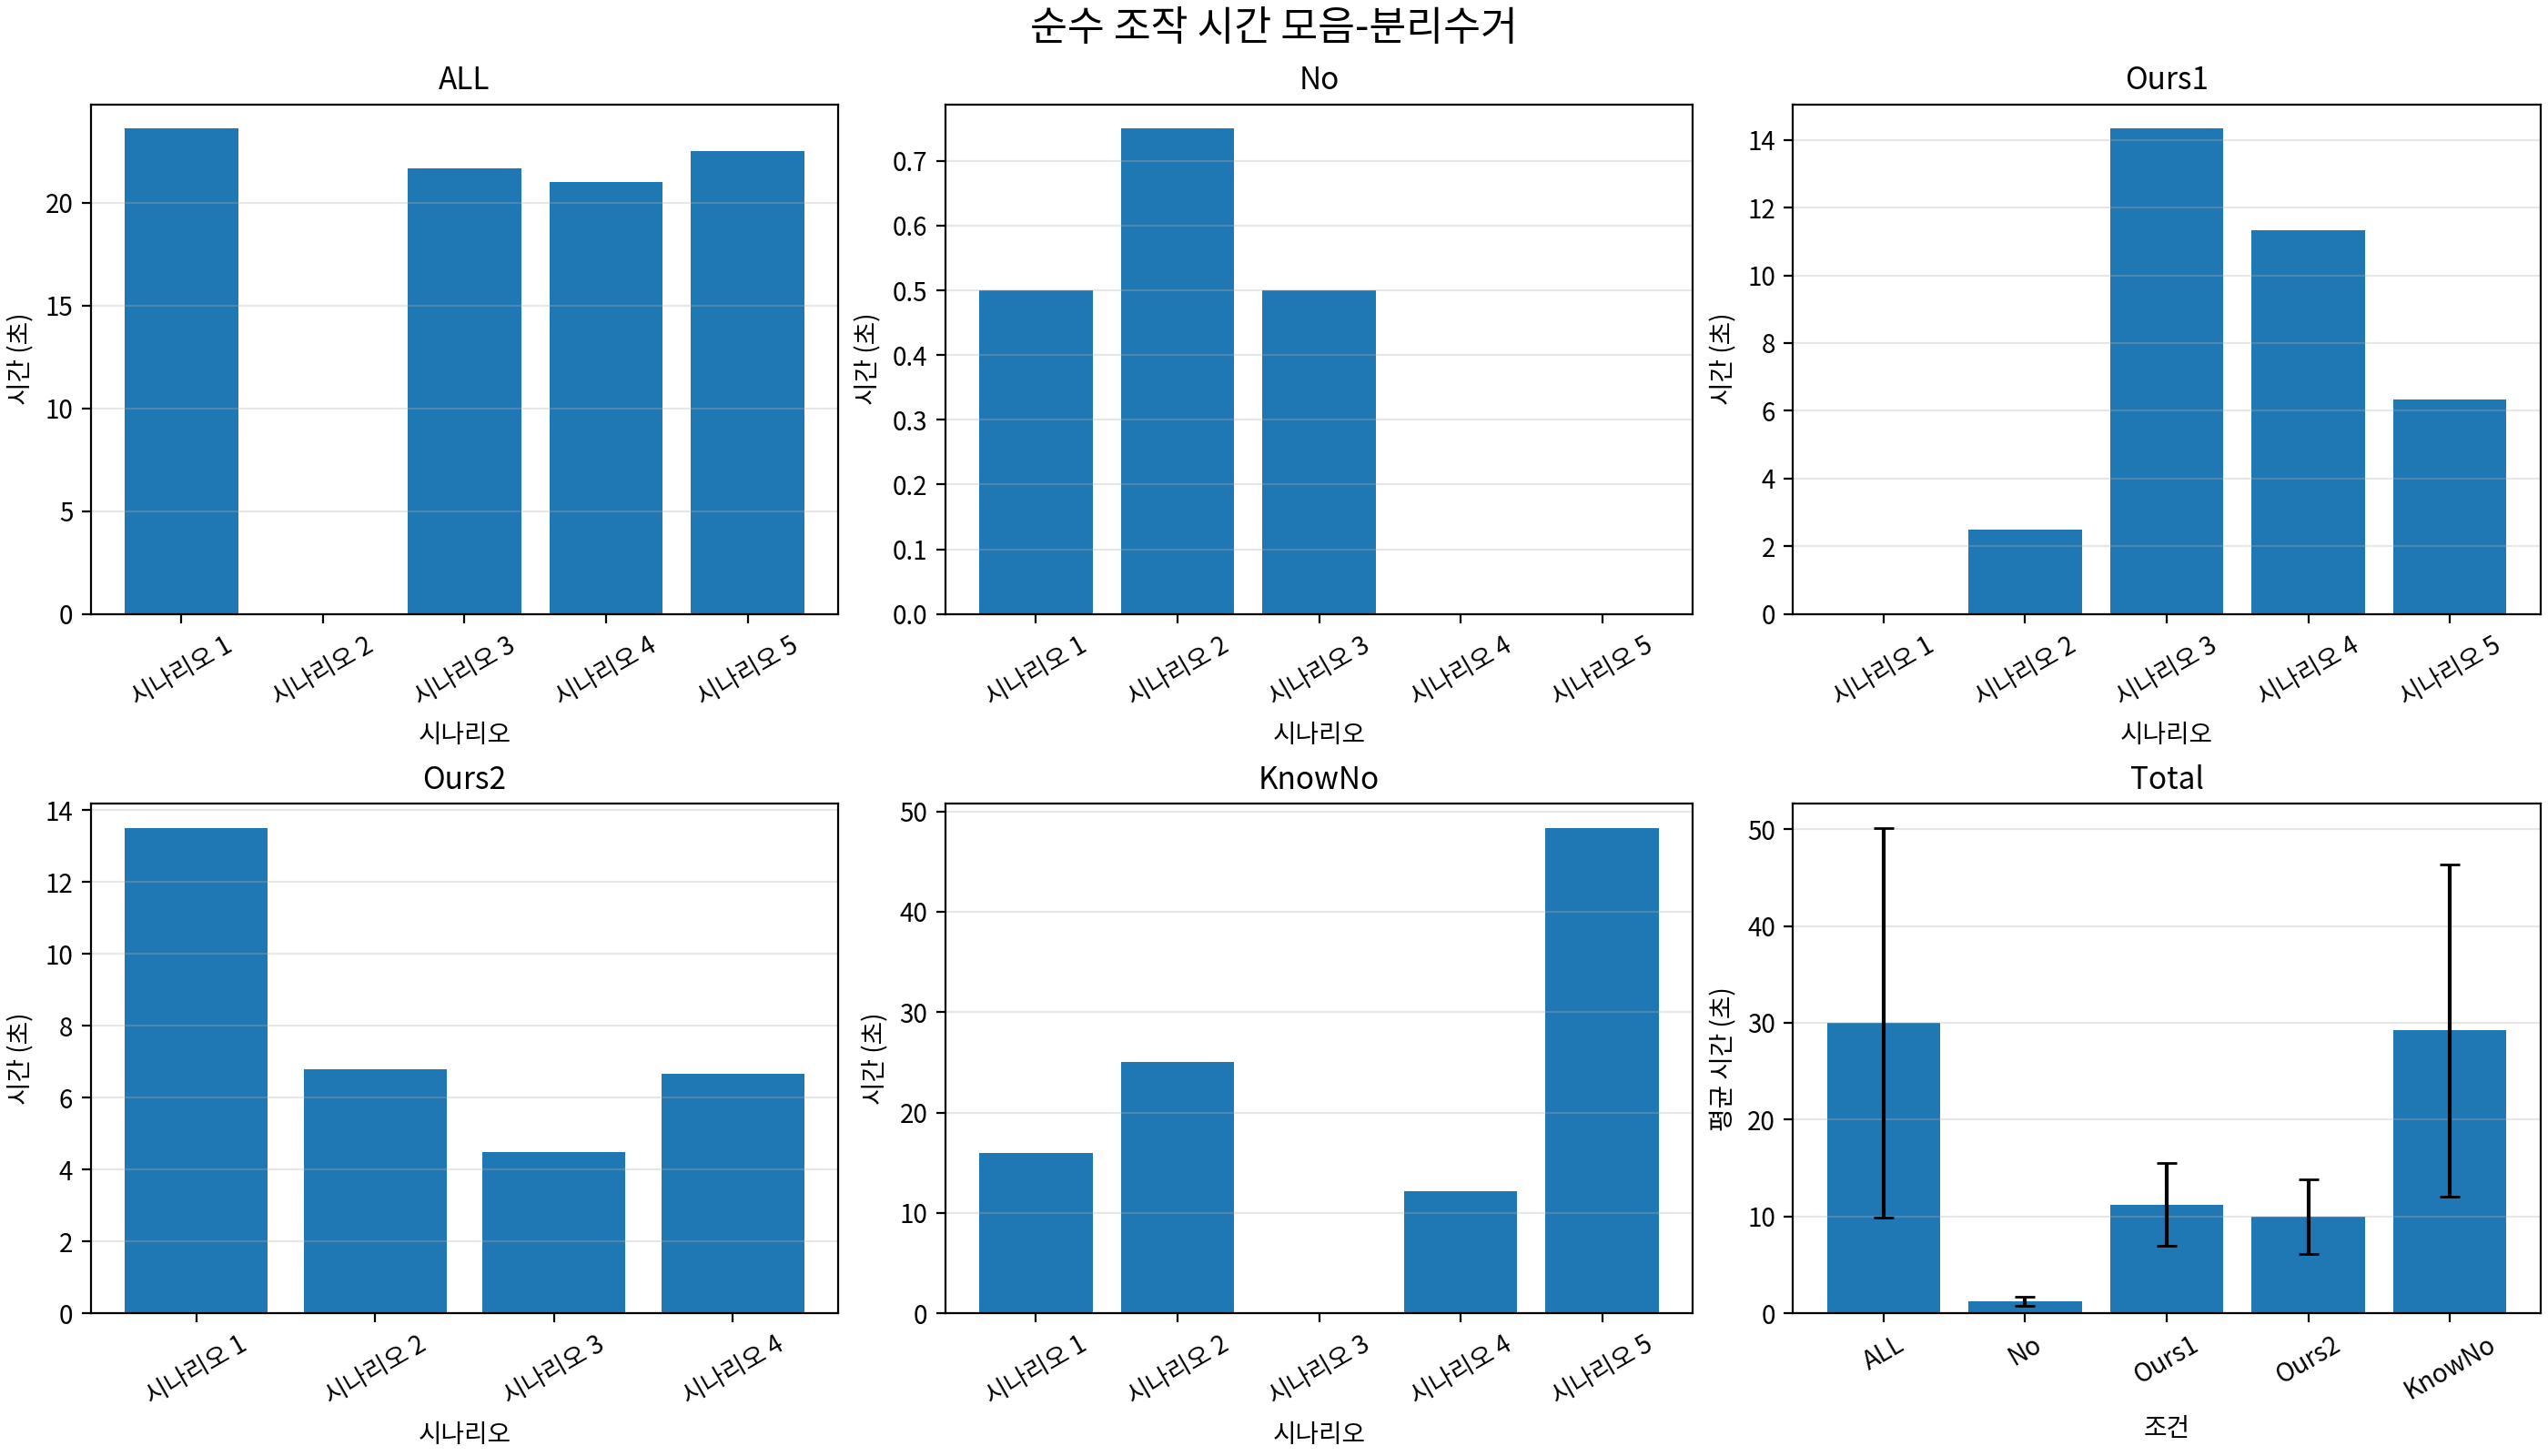
\includegraphics[width=\linewidth]{figures/fig_user_time_operation_waste.png}
        \caption{Pure operation time in waste sorting.}
        \label{fig:user_operation_waste}
    \end{subfigure}
    \hfill
    \begin{subfigure}[t]{0.49\textwidth}
        \centering
        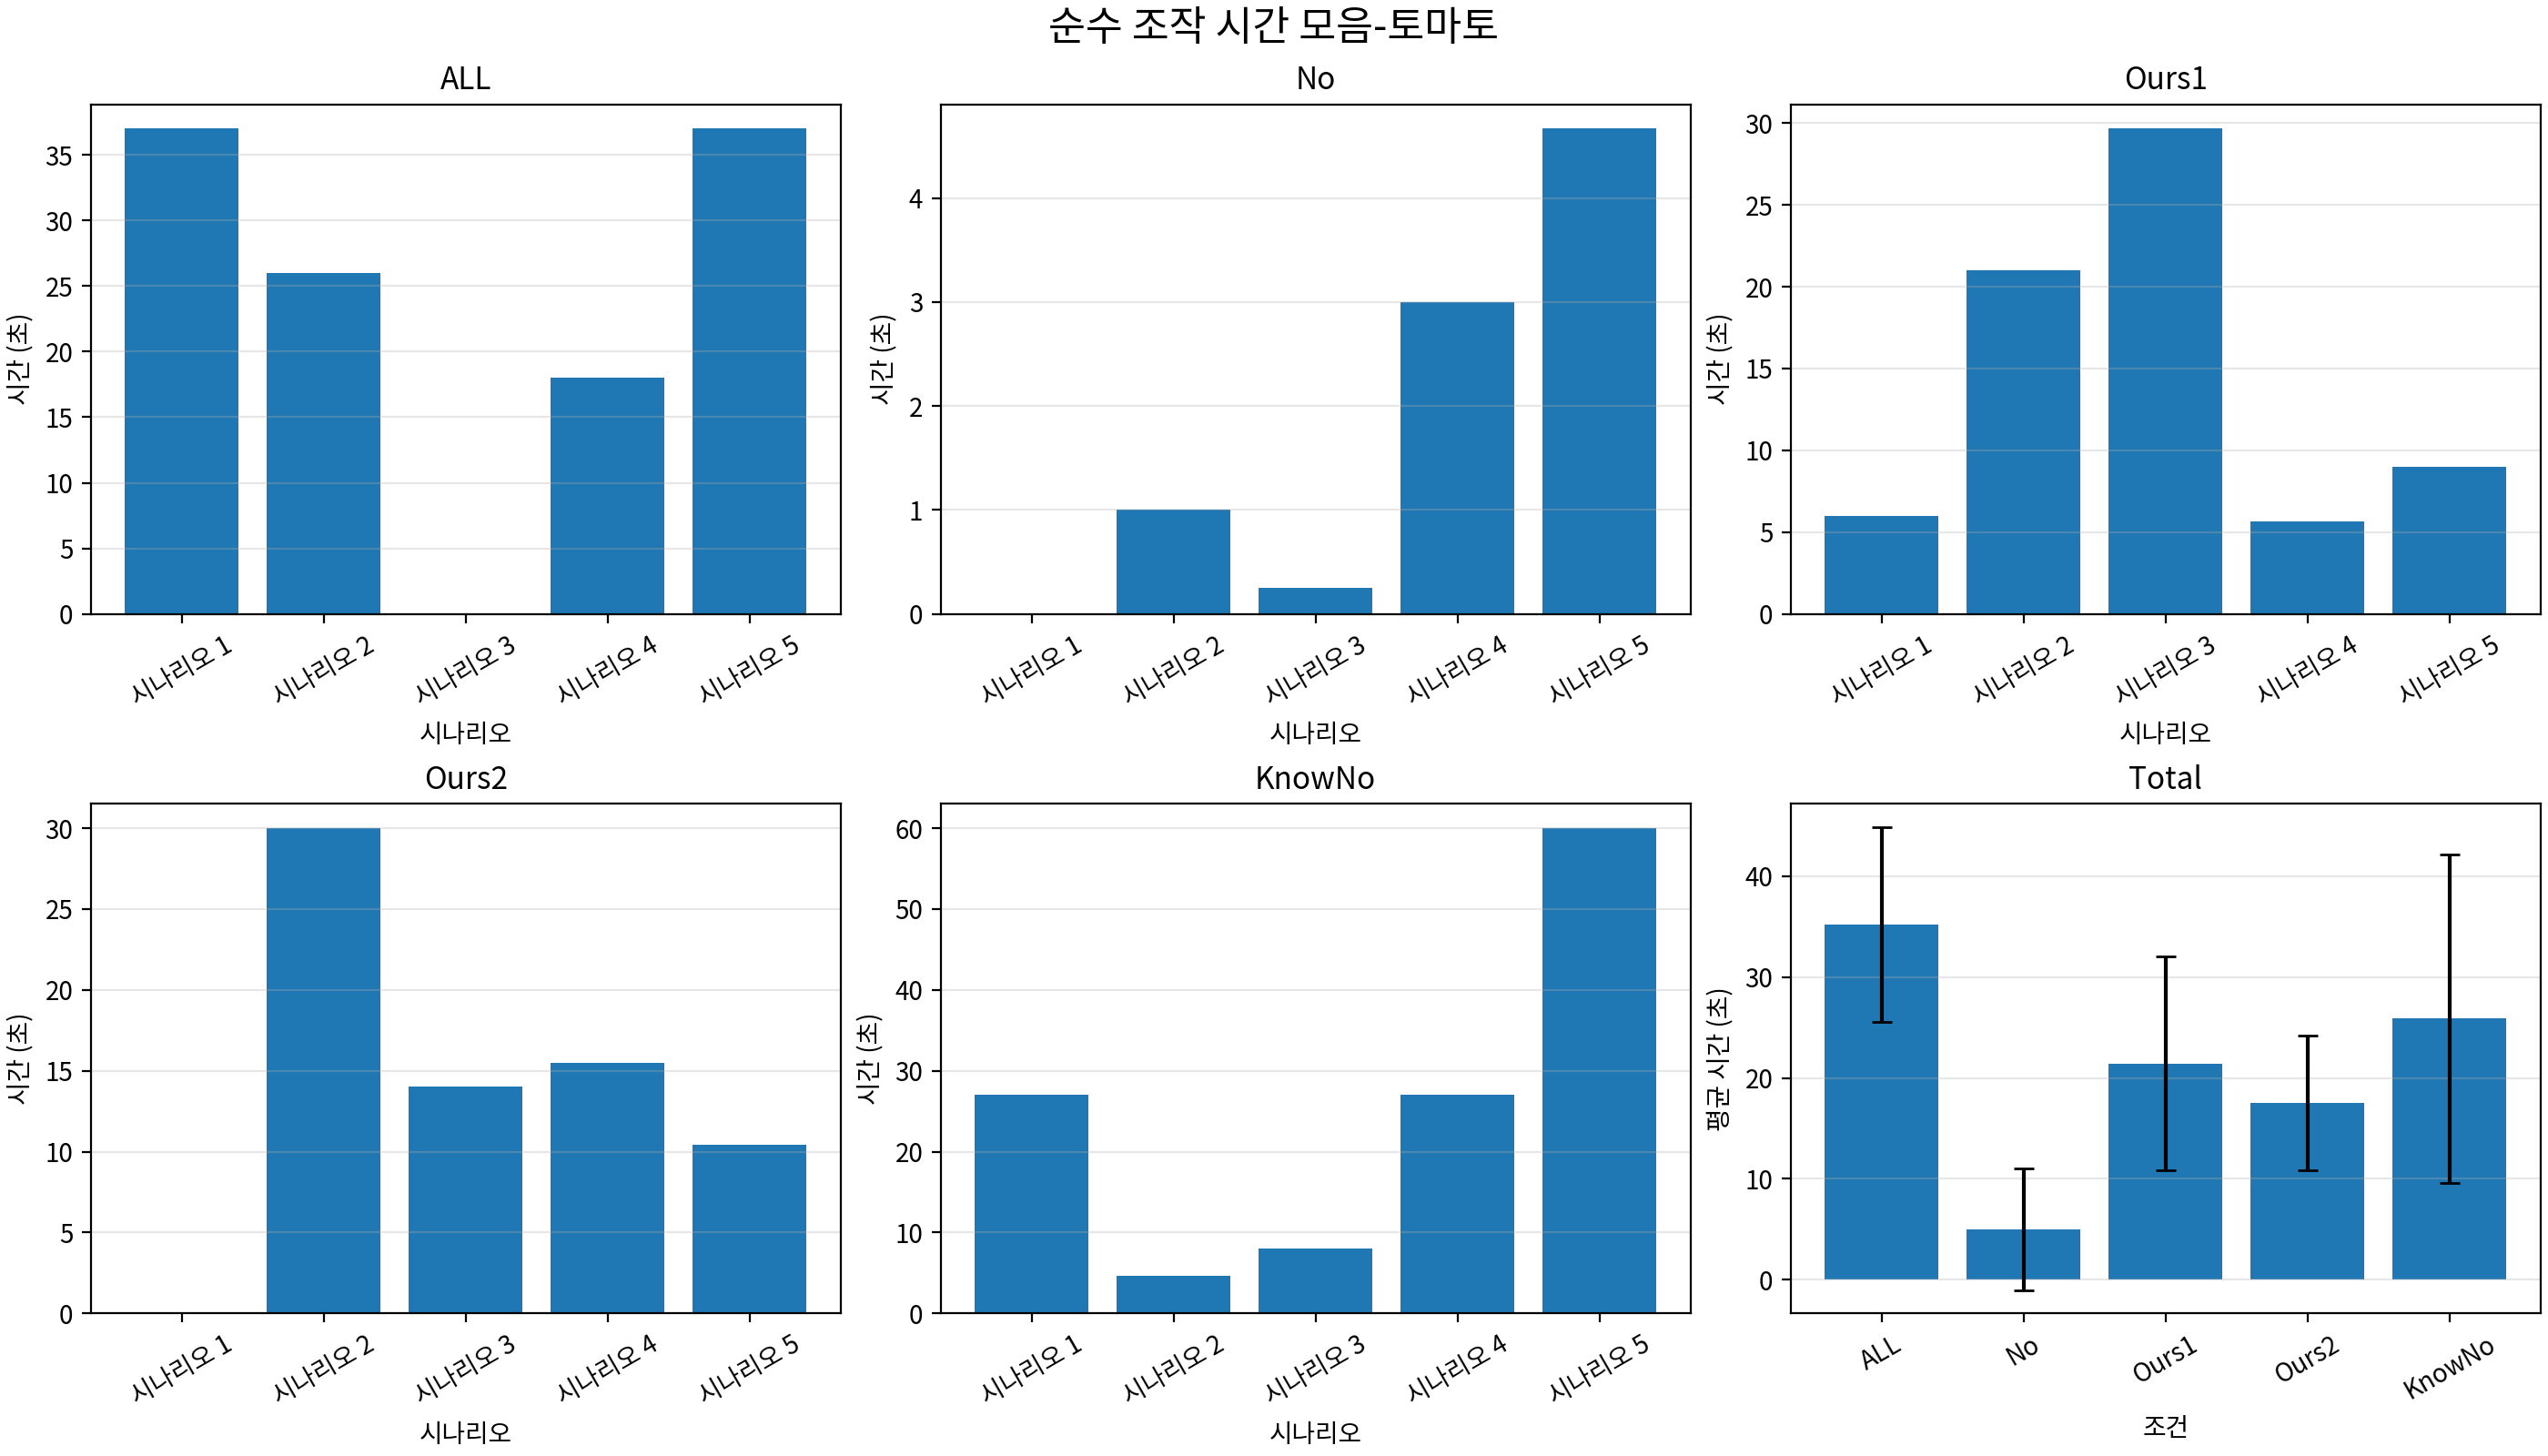
\includegraphics[width=\linewidth]{figures/fig_user_time_operation_tomato.png}
        \caption{Pure operation time in tomato harvesting.}
        \label{fig:user_operation_tomato}
    \end{subfigure}
    \vspace{0.5em}
    \begin{subfigure}[t]{0.49\textwidth}
        \centering
        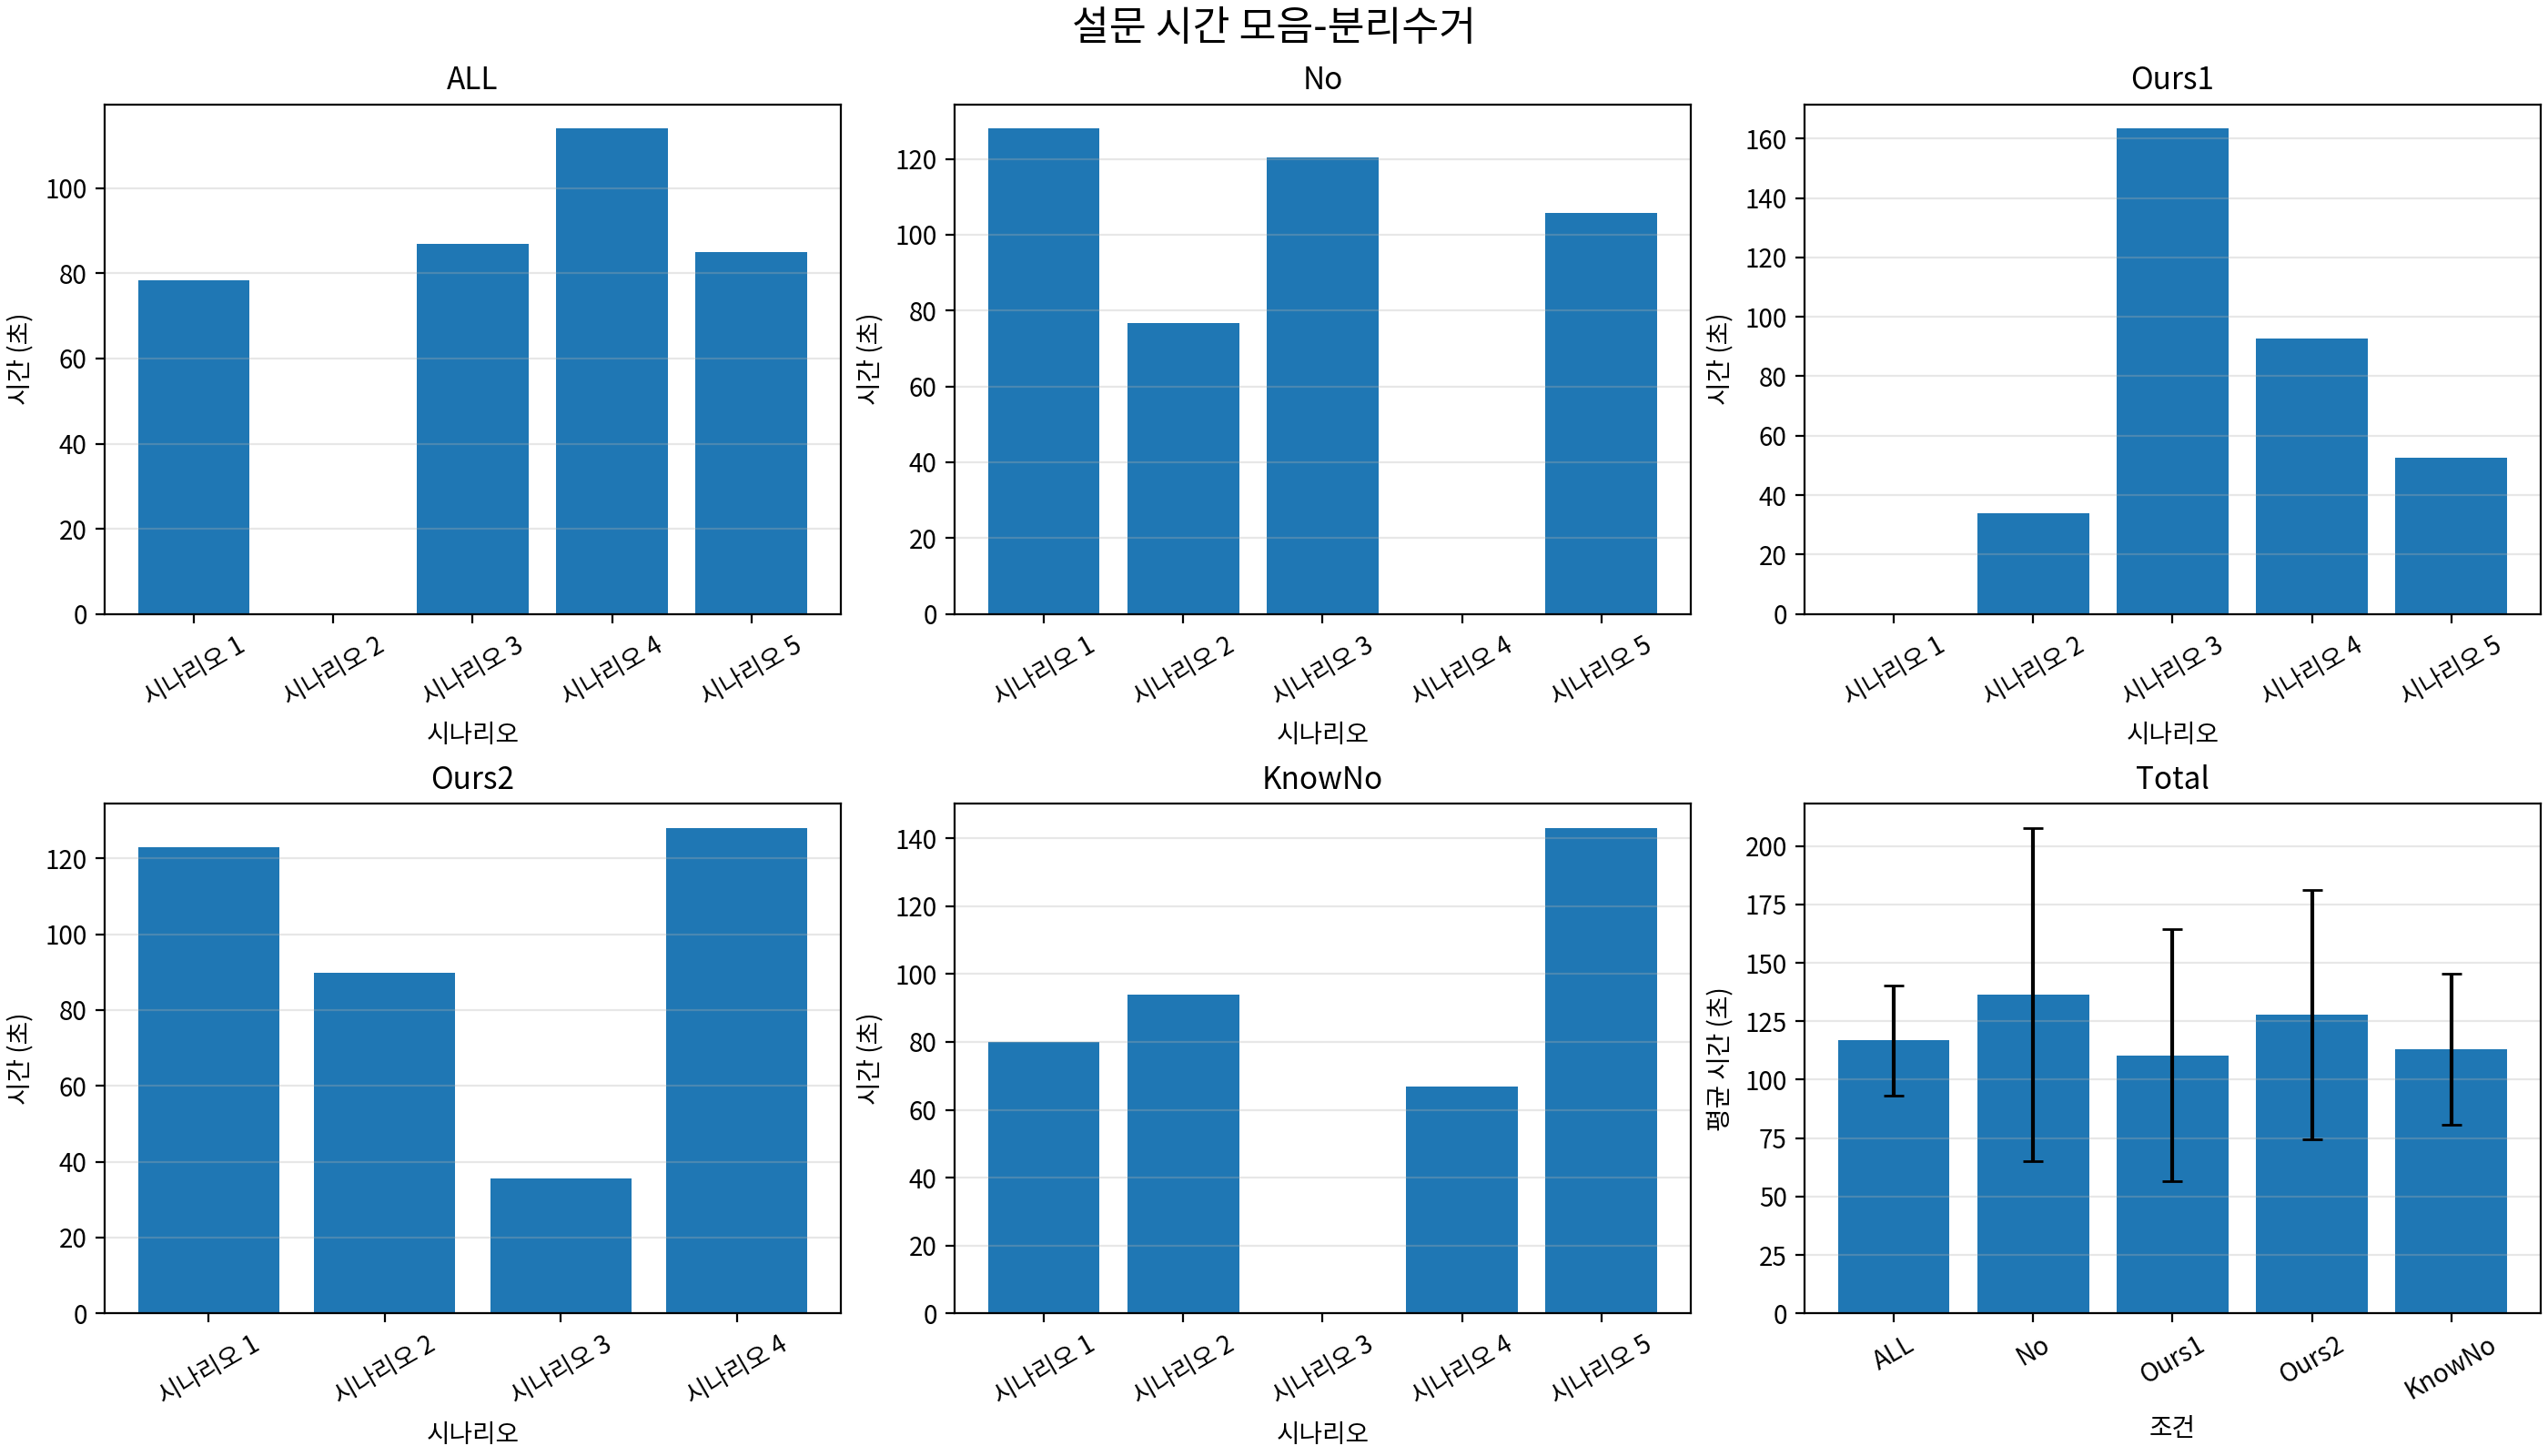
\includegraphics[width=\linewidth]{figures/fig_user_time_survey_waste.png}
        \caption{Survey time in waste sorting.}
        \label{fig:user_survey_time_waste}
    \end{subfigure}
    \hfill
    \begin{subfigure}[t]{0.49\textwidth}
        \centering
        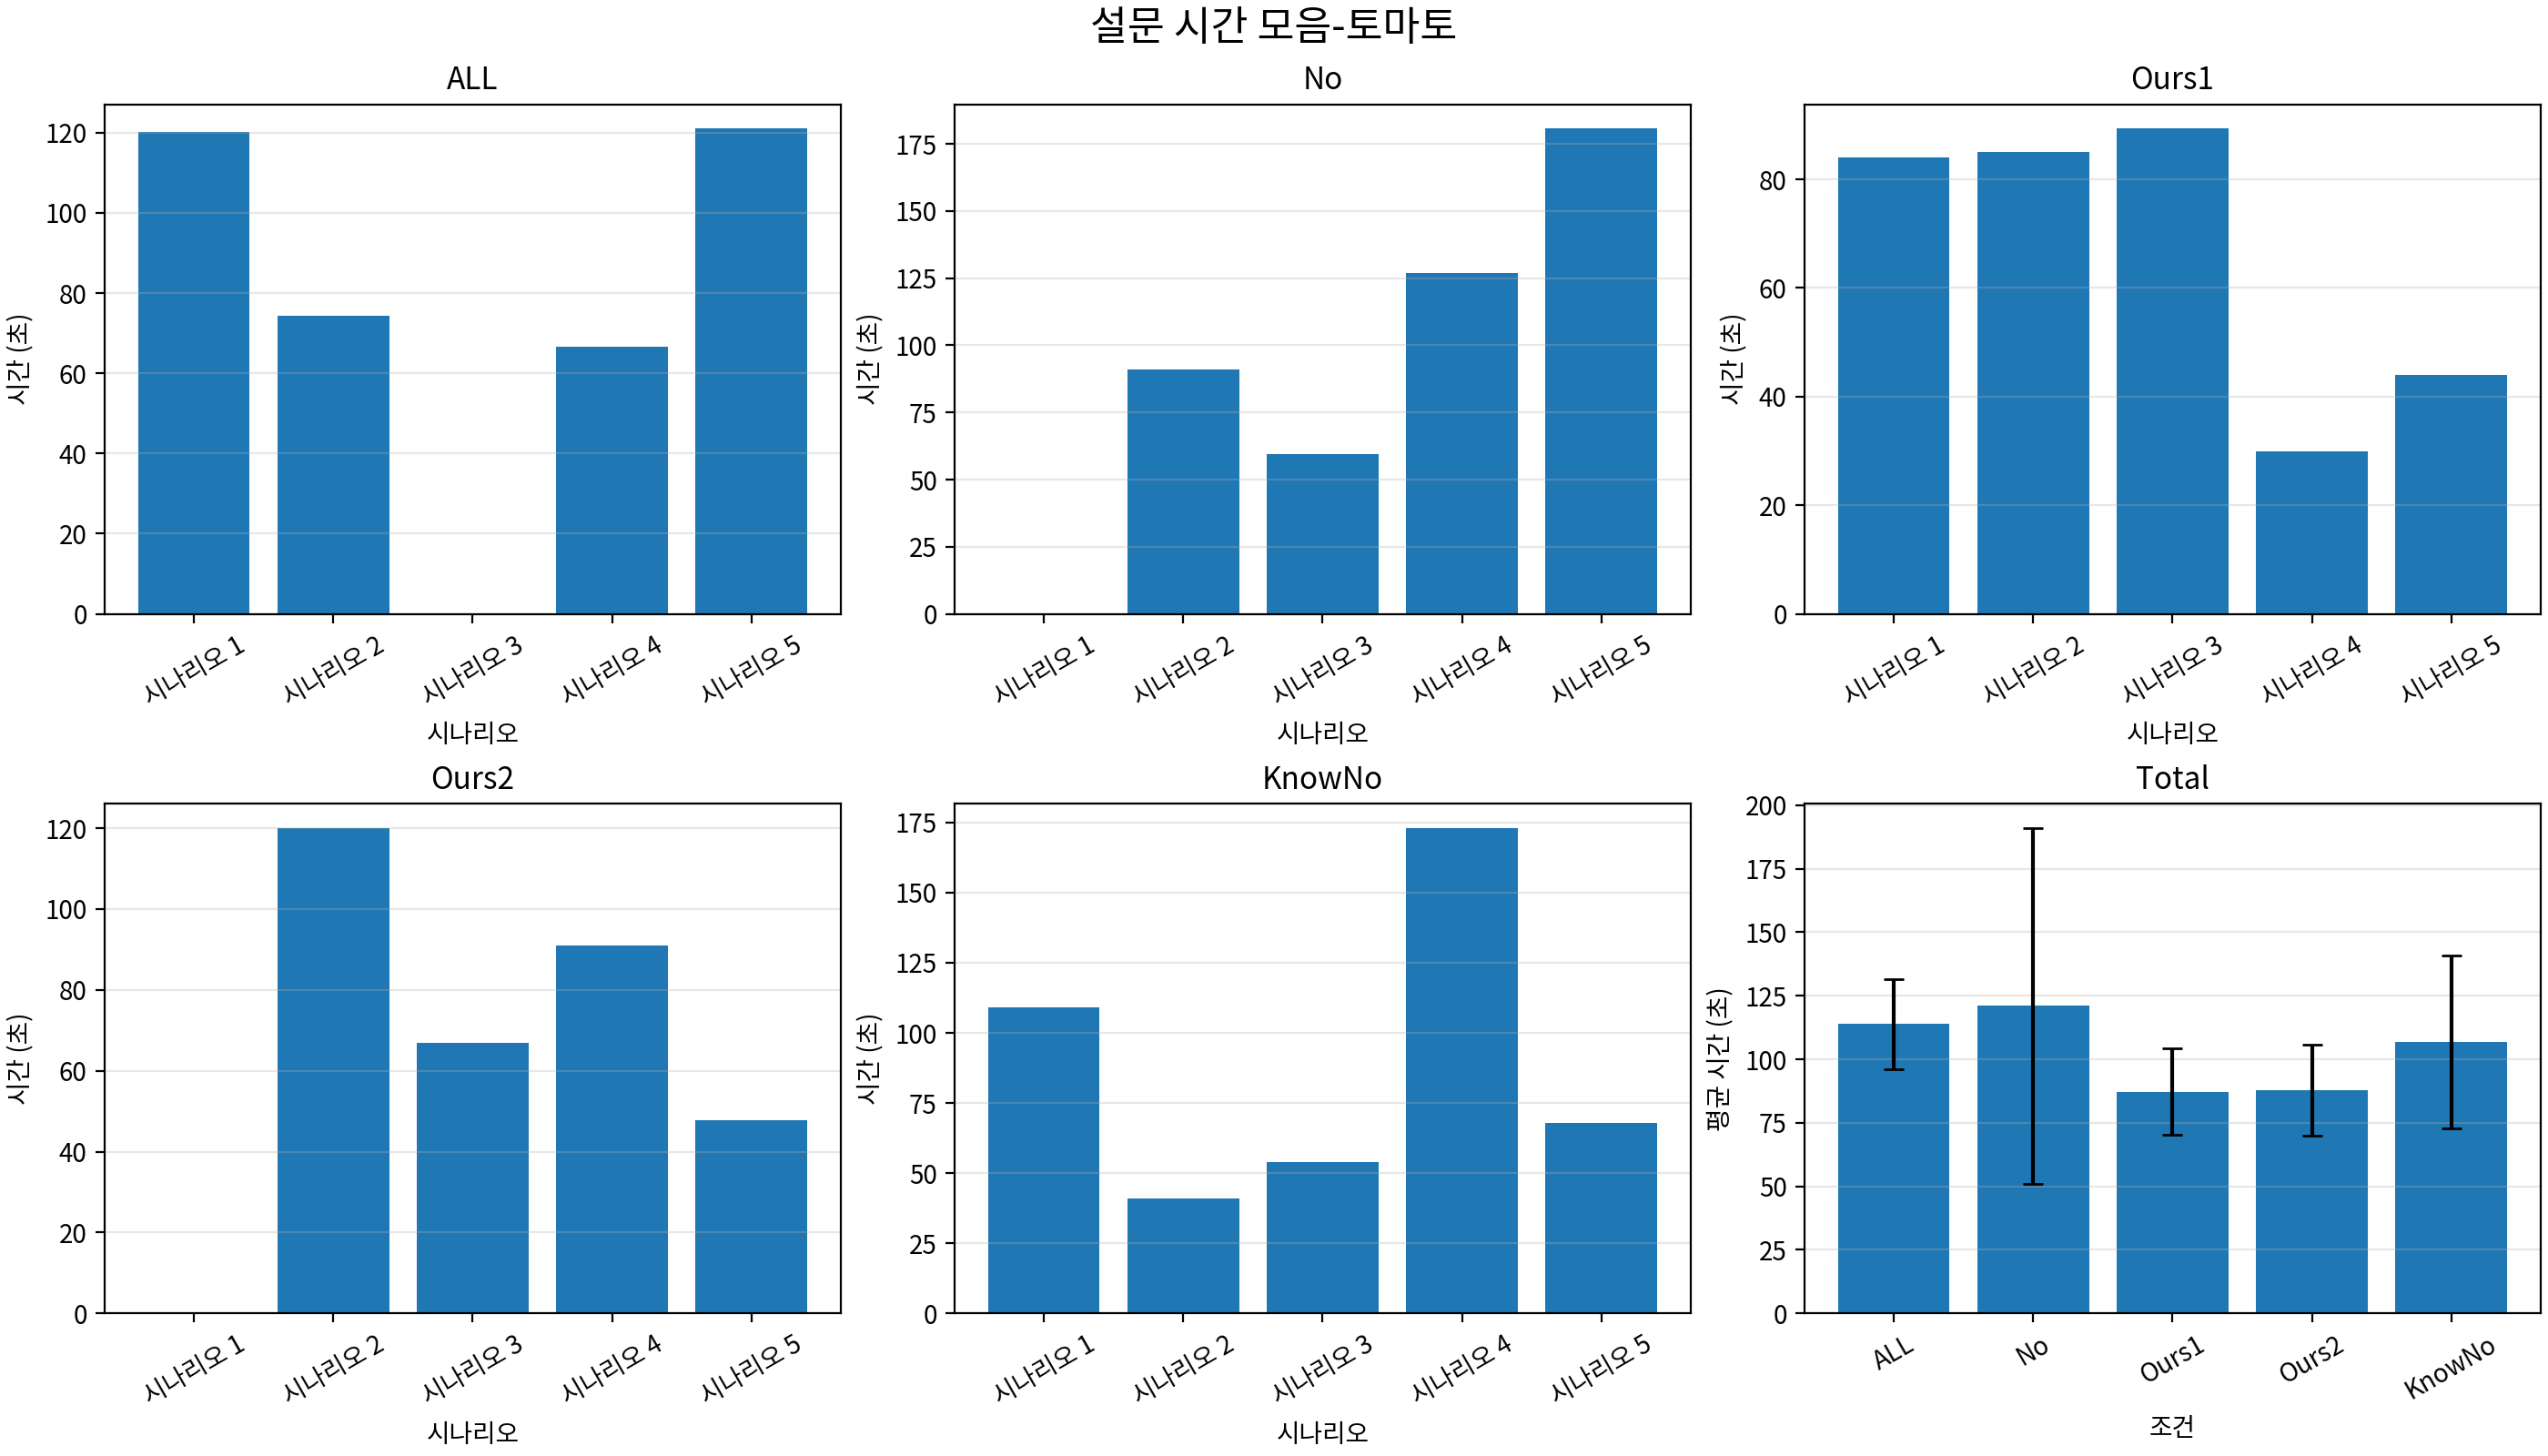
\includegraphics[width=\linewidth]{figures/fig_user_time_survey_tomato.png}
        \caption{Survey time in tomato harvesting.}
        \label{fig:user_survey_time_tomato}
    \end{subfigure}
    \caption{Time-cost results by domain. Operation time subtracts the scenario video duration and therefore reflects pure user operation time. Survey time is reported separately. Empty scenario--condition cells in the source data are retained as missing values and excluded from means.}
    \label{fig:user_time_results}
\end{figure*}

The time results separate two effects. First, selective state-level querying reduced operation time relative to continuous querying and the action-level baseline. In both domains, \textbf{Ours1} and \textbf{Ours2} required less pure operation time than \textbf{All} and \textbf{KnowNo}. Second, survey time did not follow the same ordering as operation time. In waste sorting, the average survey time was $68.53$~s for \textbf{Ours1}, $76.76$~s for \textbf{KnowNo}, $91.10$~s for \textbf{All}, $94.08$~s for \textbf{Ours2}, and $107.75$~s for \textbf{No}. In tomato harvesting, \textbf{Ours2} ($65.16$~s) and \textbf{Ours1} ($66.47$~s) were shorter than \textbf{All} ($76.45$~s), \textbf{KnowNo} ($89.00$~s), and \textbf{No} ($91.63$~s). This suggests that reducing interaction during execution does not necessarily reduce post-trial reporting time; participants may still need time to reconstruct what happened when the robot did not ask questions.

\subsubsection{Results: Situation Awareness and Subjective Burden}~\label{user:results_survey}

Fig.~\ref{fig:user_survey_results} summarizes the questionnaire results that were most relevant to the proposed query policy. In the waste sorting domain, SAGAT accuracy differed significantly across conditions, $\chi^2(4)=12.92$, $p=.012$, Kendall's $W=0.27$. \textbf{Ours1} had the highest mean accuracy ($M=0.72$, $SD=0.15$), compared with \textbf{All} ($M=0.56$, $SD=0.19$), \textbf{No} ($M=0.67$, $SD=0.07$), \textbf{Ours2} ($M=0.53$, $SD=0.12$), and \textbf{KnowNo} ($M=0.60$, $SD=0.24$). The planned comparison showed that \textbf{Ours1} was significantly higher than \textbf{All} (mean difference $=0.17$, Holm-adjusted $p=.027$, rank-biserial $r=1.00$). In tomato harvesting, the overall SAGAT condition effect was not significant, $\chi^2(4)=4.06$, $p=.398$, $W=0.08$.

\begin{figure*}[t]
    \centering
    \begin{subfigure}[t]{0.49\textwidth}
        \centering
        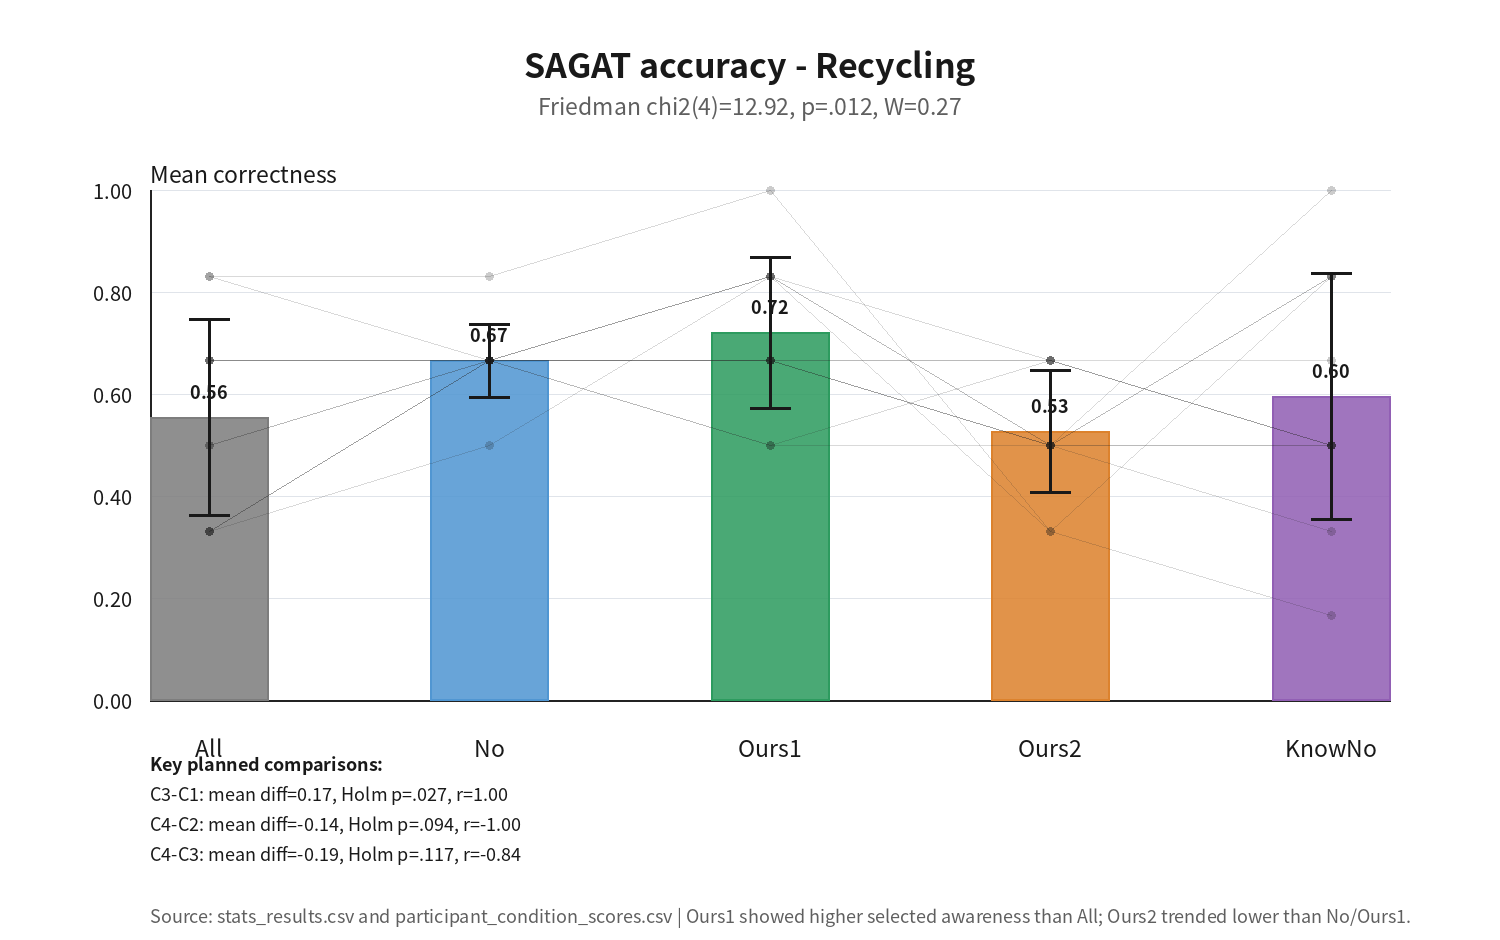
\includegraphics[width=\linewidth]{figures/fig_user_survey_sagat_accuracy_waste.png}
        \caption{SAGAT accuracy in waste sorting.}
        \label{fig:user_survey_sagat_waste}
    \end{subfigure}
    \hfill
    \begin{subfigure}[t]{0.49\textwidth}
        \centering
        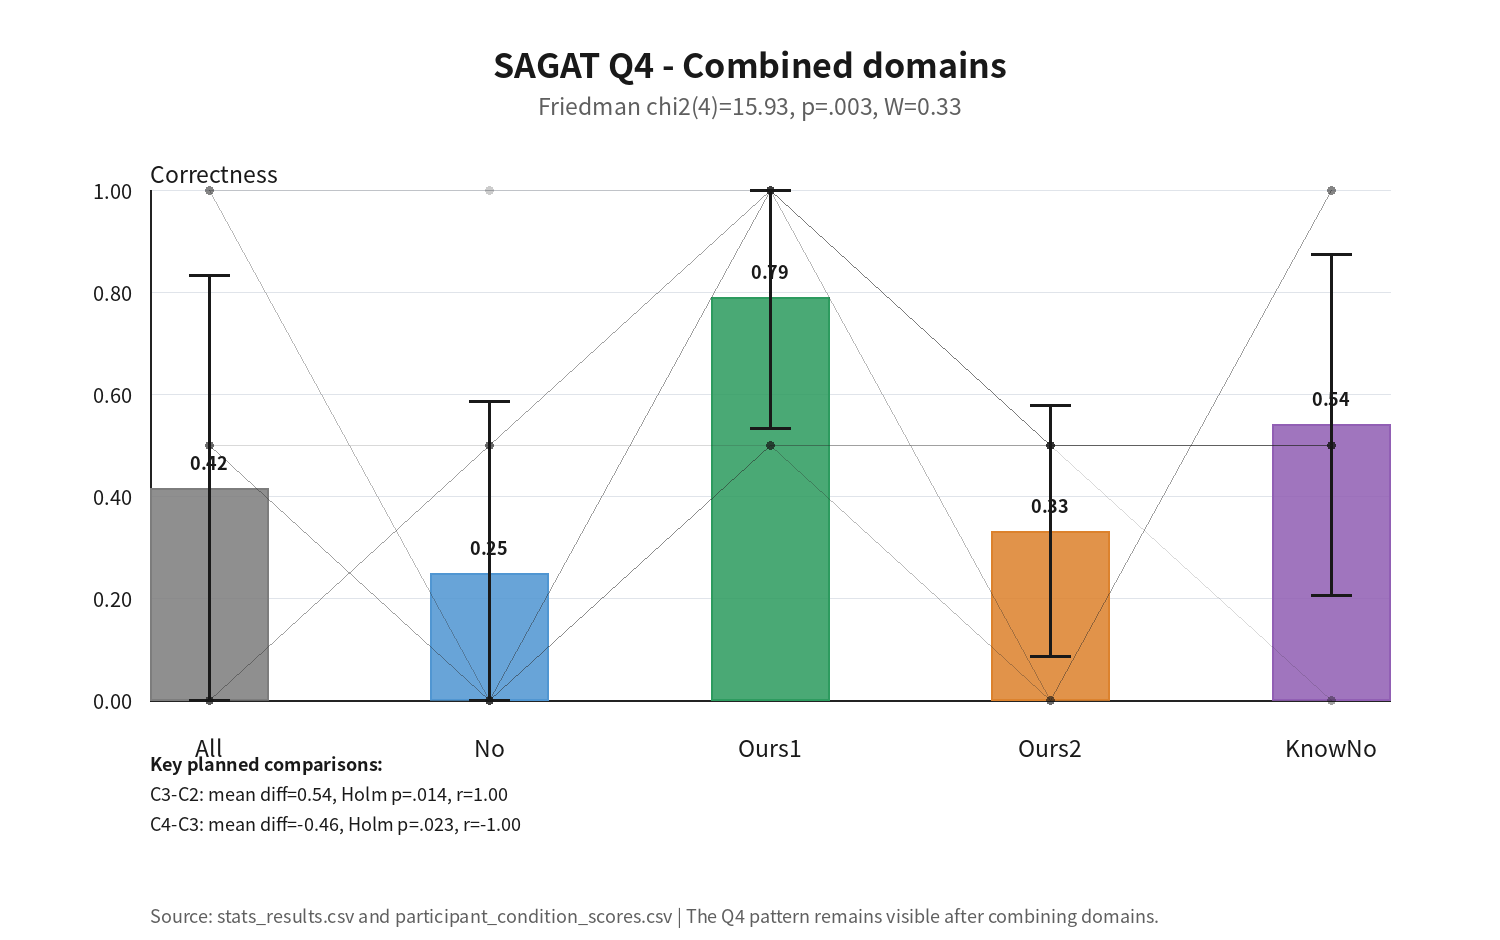
\includegraphics[width=\linewidth]{figures/fig_user_survey_sagat_q4_combined.png}
        \caption{SAGAT Q4 across both domains.}
        \label{fig:user_survey_sagat_q4}
    \end{subfigure}
    \vspace{0.5em}
    \begin{subfigure}[t]{0.49\textwidth}
        \centering
        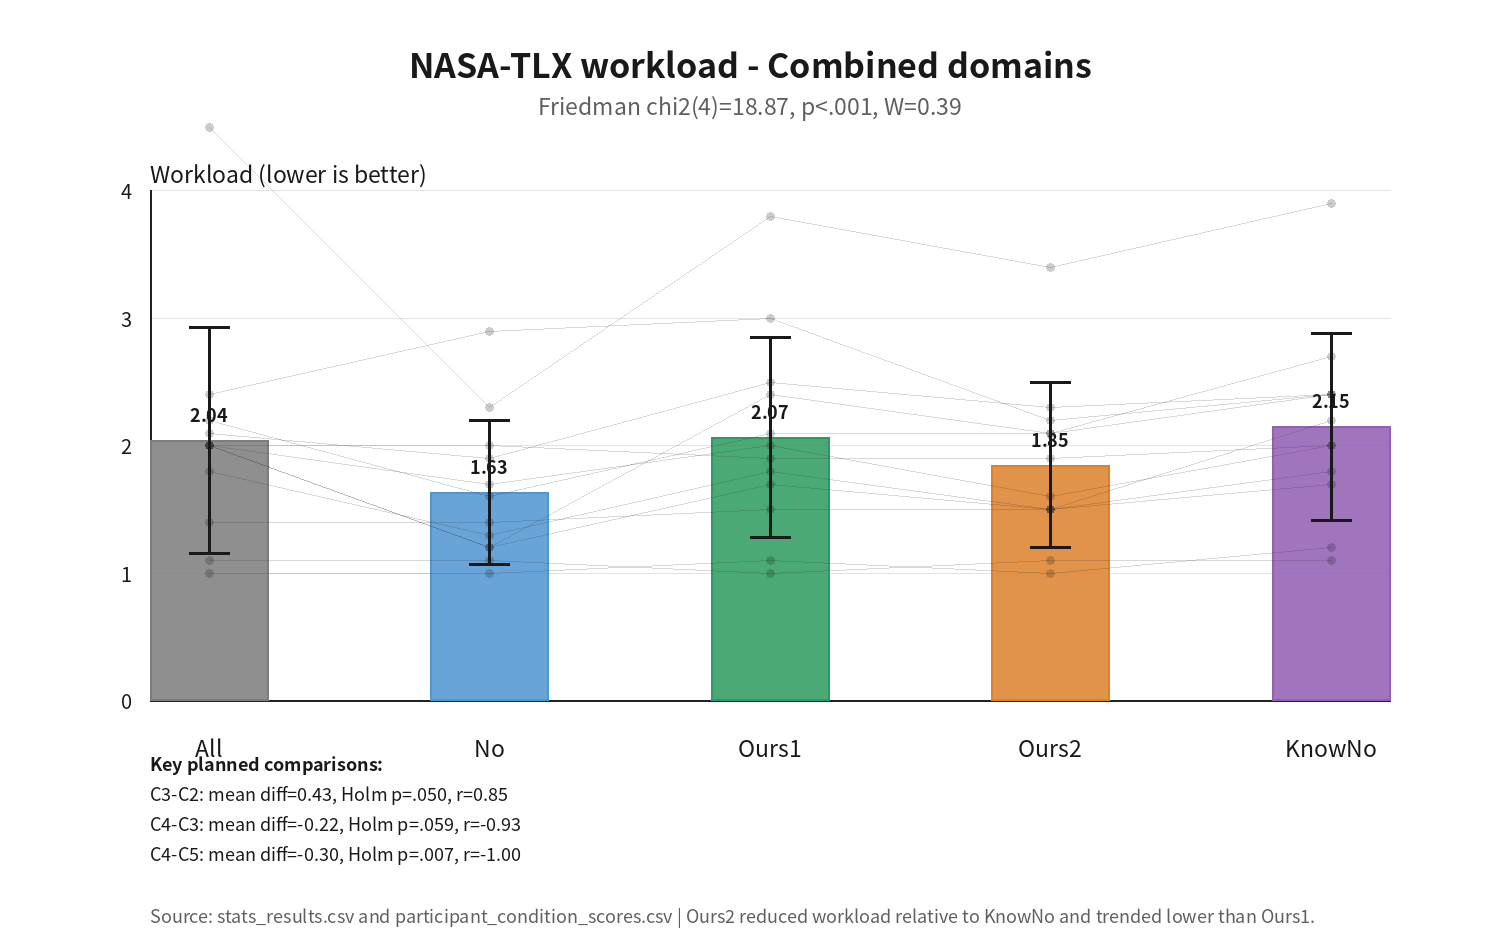
\includegraphics[width=\linewidth]{figures/fig_user_survey_workload_combined.png}
        \caption{NASA-TLX workload across both domains.}
        \label{fig:user_survey_workload}
    \end{subfigure}
    \hfill
    \begin{subfigure}[t]{0.49\textwidth}
        \centering
        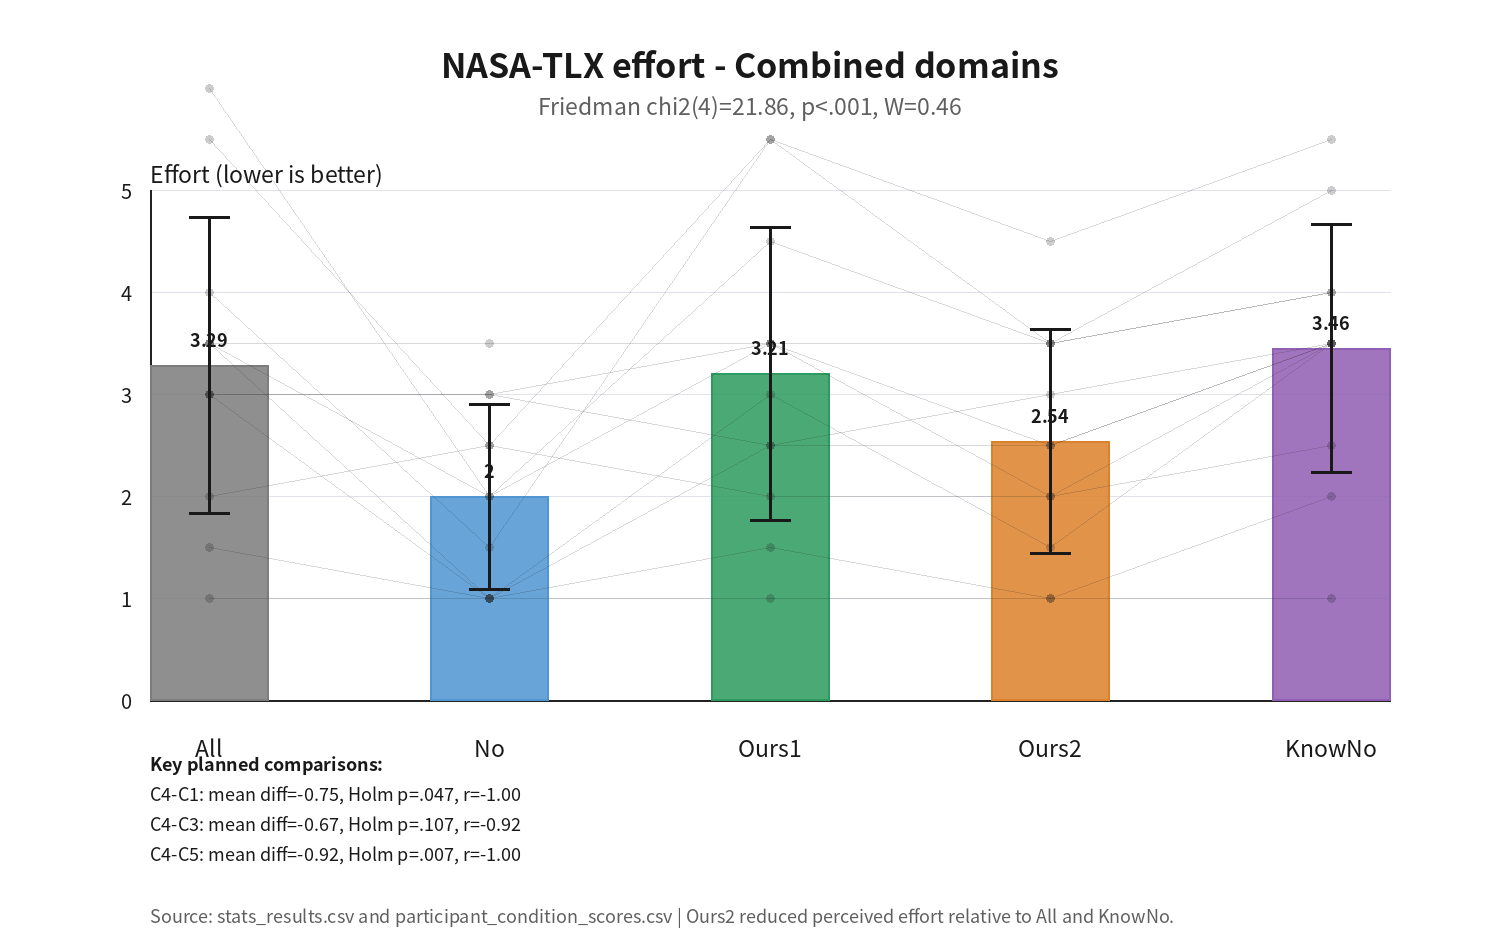
\includegraphics[width=\linewidth]{figures/fig_user_survey_effort_combined.png}
        \caption{NASA-TLX effort across both domains.}
        \label{fig:user_survey_effort}
    \end{subfigure}
    \caption{Situation-awareness and subjective-burden results. The panels report the questionnaire measures that showed the clearest condition-dependent patterns in the user study.}
    \label{fig:user_survey_results}
\end{figure*}

The strongest situation-awareness signal appeared in SAGAT Q4, which asked participants to identify why the robot requested information. In waste sorting, Q4 accuracy differed strongly across conditions, $\chi^2(4)=22.12$, $p<.001$, $W=0.46$. \textbf{Ours1} reached perfect Q4 accuracy ($M=1.00$, $SD=0.00$), outperforming \textbf{No} ($M=0.17$, $SD=0.39$; Holm-adjusted $p=.012$, $r=1.00$). \textbf{Ours2} was lower than \textbf{Ours1} ($M=0.08$ vs. $1.00$; Holm-adjusted $p=.007$, $r=-1.00$). The same Q4 pattern remained visible after combining both domains, $\chi^2(4)=15.93$, $p=.003$, $W=0.33$: \textbf{Ours1} exceeded \textbf{No} (mean difference $=0.54$, Holm-adjusted $p=.014$), while \textbf{Ours2} was lower than \textbf{Ours1} (mean difference $=-0.46$, Holm-adjusted $p=.023$).

Subjective burden showed a different pattern. NASA-TLX workload differed significantly across conditions in the aggregated data, $\chi^2(4)=18.87$, $p<.001$, $W=0.39$. \textbf{Ours2} produced lower workload ($M=1.85$, $SD=0.64$) than \textbf{KnowNo} ($M=2.15$, $SD=0.73$; Holm-adjusted $p=.007$, $r=-1.00$), and also trended lower than \textbf{Ours1} ($M=2.07$, $SD=0.79$; Holm-adjusted $p=.059$, $r=-0.93$). Effort followed the same direction, $\chi^2(4)=21.86$, $p<.001$, $W=0.46$. \textbf{Ours2} required less effort than \textbf{All} ($M=2.54$ vs. $3.29$; Holm-adjusted $p=.047$, $r=-1.00$) and \textbf{KnowNo} ($M=2.54$ vs. $3.46$; Holm-adjusted $p=.007$, $r=-1.00$). In waste sorting, \textbf{Ours2} also reduced effort relative to \textbf{KnowNo} ($M=2.58$ vs. $4.00$; Holm-adjusted $p=.014$, $r=-1.00$).

\subsubsection{Discussion}~\label{user:discussion}

The three analysis axes show that query timing and query content affect different aspects of the interaction. The response-quality analysis indicates that state-level queries can support accurate answers, especially when evaluated at the stricter task level. \textbf{Ours2} achieved perfect task success in the first three scenarios and remained substantially higher than \textbf{KnowNo} in the later scenarios. This result is consistent with the planning motivation of the proposed method: instead of asking the user to choose the robot's next action, the robot asks about a state hypothesis that resolves task-relevant uncertainty.

The time analysis shows the practical cost of each interaction strategy. As expected, \textbf{No} minimized operation time because the user had almost nothing to do during execution. This does not make \textbf{No} a desirable collaborative strategy, because it removes the user's ability to correct robot uncertainty. Among the interactive conditions, \textbf{Ours1} and \textbf{Ours2} reduced pure operation time relative to \textbf{All} and \textbf{KnowNo} in both domains. This suggests that selective state-level querying can reduce the direct time cost of human intervention compared with continuous supervision and action-level questioning.

The questionnaire analysis clarifies the awareness--burden tradeoff. \textbf{Ours1} produced the clearest situation-awareness benefit, especially for SAGAT Q4. This suggests that uncertainty-triggered state queries can make the reason for robot uncertainty more legible to the user. However, \textbf{Ours1} did not reduce workload as consistently as \textbf{Ours2}. In contrast, \textbf{Ours2} reduced workload and effort relative to \textbf{KnowNo}, but did not reproduce the same Q4 advantage as \textbf{Ours1}. Thus, the two variants should not be interpreted as a simple winner-loser comparison. \textbf{Ours1} emphasizes selected awareness at critical uncertainty points, whereas \textbf{Ours2} distributes queries across a broader set of situations and produces lower subjective burden.

These results support the central claim that human feedback should be treated as a limited resource in robot planning. Asking at every opportunity can preserve supervision but increases interaction cost. Asking no questions minimizes immediate burden but gives the robot no opportunity to repair uncertain beliefs. Asking action-level questions can shift planning responsibility to the user. The proposed state-level querying approach offers a middle ground: it asks only when belief uncertainty is high and frames the question around the state information needed by the planner.

The study also has limitations. The sample size was small, and several effects should be interpreted as descriptive or exploratory even when the direction is consistent. The SAGAT benefit of \textbf{Ours1} was concentrated in waste sorting and especially in Q4, so it should be described as an improvement in selected awareness measures rather than a general improvement in all aspects of situation awareness. Finally, the WoZ protocol controlled the interaction sequence and isolated the user-side effect of the query policy; deployment in a fully autonomous system requires the system-level reliability evaluated separately in Section~\ref{exp:sys_eval}.
